\documentclass[border=10pt]{standalone}

\usepackage{tikz}
\usepackage{tikzsymbols}
\usetikzlibrary{calc,patterns,shapes.geometric}

\def\centerarc[#1](#2)(#3:#4:#5){\draw[#1] ($(#2)+({#5*cos(#3)},{#5*sin(#3)})$) arc (#3:#4:#5);}

\begin{document}
	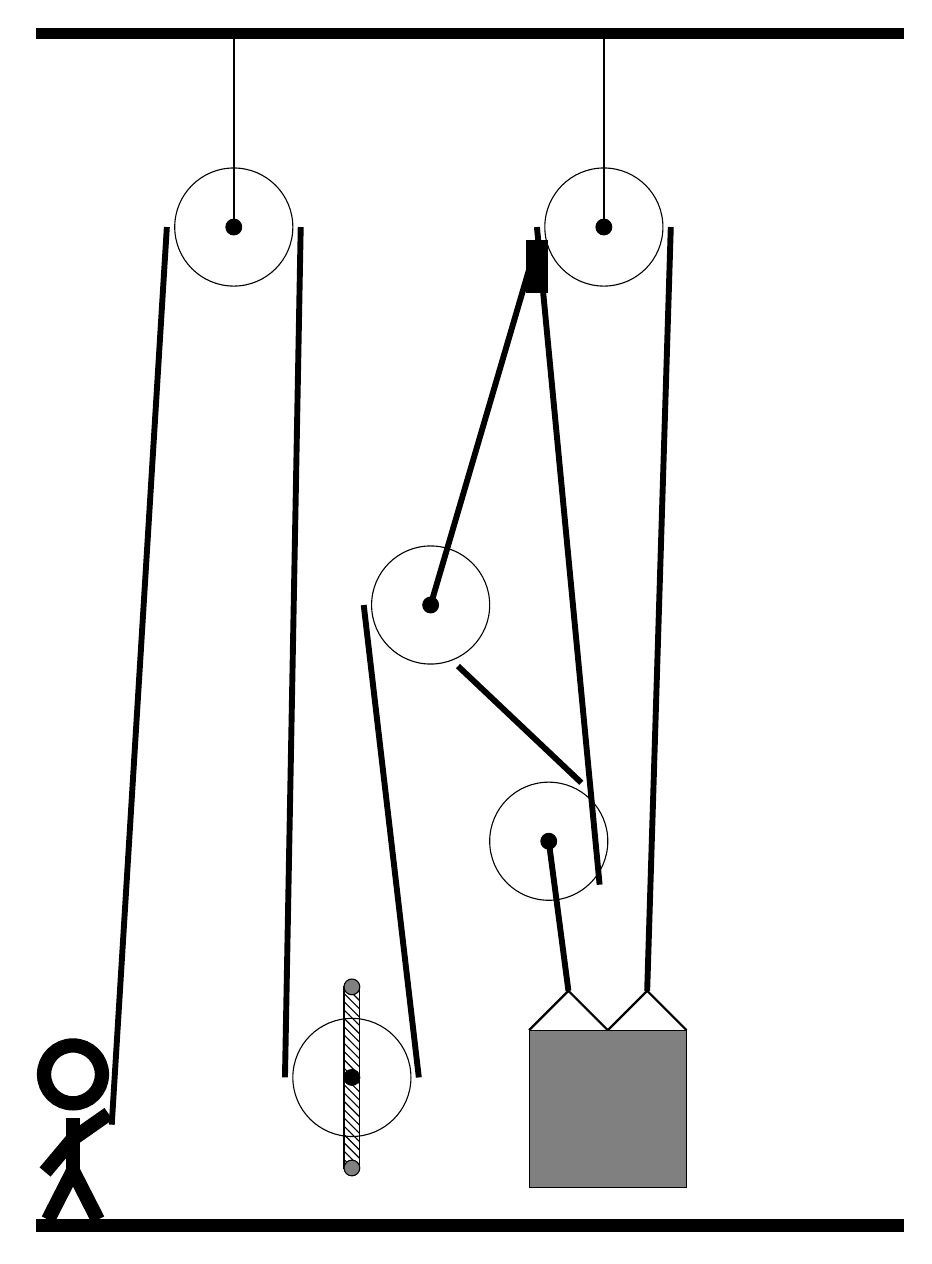
\begin{tikzpicture}
		%%%%% START %%%%%
		\draw[fill=black] (-6, 12) rectangle (5, 12.125);
		
		\draw (-1, 4.8) circle (0.75);
		\draw[fill=black] (-1, 4.8) circle (0.1);
		
		\draw (0.5, 1.8) circle (0.75);
		\draw[fill=black] (0.5, 1.8) circle (0.1);
		
		\draw (1.2, 9.6) circle (0.75);
		\draw[fill=black] (1.2, 9.6) circle (0.1);
		\draw[thick] (1.2, 9.6) -- (1.2, 12);
		
		\draw (-3.5, 9.6) circle (0.75);
		\draw[fill=black] (-3.5, 9.6) circle (0.1);
		\draw[thick] (-3.5, 9.6) -- (-3.5, 12);
		
		\draw (-2, -1.2) circle (0.75);
		\draw[fill=black] (-2, -1.2) circle (0.1);
		\draw[pattern=north west lines, pattern color=black] (-2.1, -0.05) rectangle (-1.9, -2.35);
		\draw[fill=black!50] (-2, -0.05) circle (0.1);
		\draw[fill=black!50] (-2, -2.35) circle (0.1);
		
		\draw[thick]  (0.25, -0.6) -- (0.75, -0.1) -- (1.25, -0.6) -- (1.75, -0.1) -- (2.25, -0.6);
		\draw[fill=black!50] (0.25, -0.6) rectangle (2.25, -2.6);
		\draw[line width=0.75mm] (-5.05, -1.8) -- (-4.35, 9.6);
		\centerarc[line width=0.75mm](-3.5, 9.6)(0:180:0.85);
		\draw[line width=0.75mm] (-2.65, 9.6) -- (-2.85, -1.2);
		\centerarc[line width=0.75mm](-2, -1.2)(180:360:0.85);
		\draw[line width=0.75mm] (-1.15, -1.2) -- (-1.85, 4.8);
		\draw[line width=0.75mm] (-1, 4.8) -- (0.35, 9.4);
		\draw[line width=0.75mm, fill=black](0.25, 8.8) rectangle (0.45, 9.4);
		\centerarc[line width=0.75mm](-1, 4.8)(-20:180:0.85);
		\draw[line width=0.75mm] (-0.653, 4.024) -- (0.914, 2.542);
		\centerarc[line width=0.75mm](0.5, 1.8)(160:380:0.85);
		\draw[line width=0.75mm] (1.146, 1.248) -- (0.35, 9.6);
		\draw[line width=0.75mm](0.5, 1.8) -- (0.75, -0.1);
		\centerarc[line width=0.75mm](1.2, 9.6)(0:180:0.85);
		\draw[line width=0.75mm] (2.05, 9.6) -- (1.75, -0.1);
		
		\node at (-5.5, -1.9) {\Strichmaxerl[10][50][35]};
		
		\draw[fill=black] (-6, -3) rectangle (5, -3.15);
		%%%%% END %%%%%
	\end{tikzpicture}
\end{document}